\section{HTML básico}

Las etiquetas que siempre debe contener un documento \textit{.html} o \textit{.htm} son:
\begin{lstlisting}
    <html>
        <head>
        </head>
        <body>
            This is a line of text.
        </body>
    </html>
\end{lstlisting}


\subsection{Tipos de etiquetas}
\begin{itemize}
    \item \textbf{Block-levels}: establecen una estructura o característica primordial dentro de la estructura HTML, suelen ser la cabecera o contenedor de otras etiquetas, y dan un salto de línea cuando estas etiquetas se cierran.
    \item \textbf{Inline}: son aquellas etiquetas que no van dentro de otras para dar formato al contenido de las mismas, y no dan un salto de línea cuando se cierran.
    \item Existen elementos que son Block-level e Inline, algunos ejemplos son:
    \begin{itemize}
        \item \textbf{applet}: subprograma Java embebido.
        \item \textbf{iframe}: estructura frame.
        \item \textbf{ins}: texto insertado.
        \item \textbf{map}: mapa de imagen.
        \item \textbf{object}: objetos embebidos.
        \item \textbf{scritp}: un script dentro del documento HTML.
    \end{itemize}
    \item Los elementos Inline no pueden contener elementos Block-level.
\end{itemize}


\subsection{Etiquetas básicas de HTML}
\begin{itemize}
    \item \textbf{p}: agrega un párrafo de texto al sitio o página.
    \item \textbf{span}: contiene texto en el sitio o página.
    \item \textbf{h, h1 h2, ..., h6}: agrega un título 1, título 2, ..., hasta título 6 al sitio o página. No es recomendable utilizar los títulos solamente para hacer grande el texto, ya que los buscadores los utilizan para indexar el sitio o página con la web.
    \item \textbf{title}: es el título de la pestaña del sitio o página.
    \item \textbf{hr/}: crea una línea horizontal. \textbf{No requiere de una etiqueta de comienzo.}
    \item \textbf{br/}: agrega un espacio en blanco o salto de línea. \textbf{No requiere de una etiqueta de comienzo}.
    \item \textbf{div}: es un elemento Block-level que suele ser utilizado para contener otras etiquetas.
\end{itemize}

Un ejemplo del aspecto de las etiquetas anteriormente mencionadas es el siguiente código y la \textit{Figura \ref{fig: 1}}:
\begin{lstlisting}
    <!-- Tipos de encabezados. -->
    <h1>Título 1</h1>
    <h2>Título 1.1</h2>
    <h3>Título 1.1.1</h3>
    <h4>Título 1.1.1.1</h4>
    <h5>Título 1.1.1.1.1</h5>
    <h6>Título 1.1.1.1.1.1</h6>

    <!-- Etiquetas para objetos. -->
    <p>Esto es un párrafo, contenido en un P,<br/>acabo de dar un salto de línea con BR.</p>
    <span>Esto es otro párrafo, contenido en un SPAN.</span>
    
    <!-- Salto de línea. -->
    <hr/>
    
    <!-- Contenedor que almacena un párrafo. -->
    <div>
        <p>Esto es otro párrafo, separado de los demás con una línea horizontal HR; contenido en un P dentro de un contenedor DIV.</p>
    </div>
\end{lstlisting}
\begin{figure}[H]
    \centering
    \caption{Vista de las etiquetas básicas}
    \label{fig: 1}
    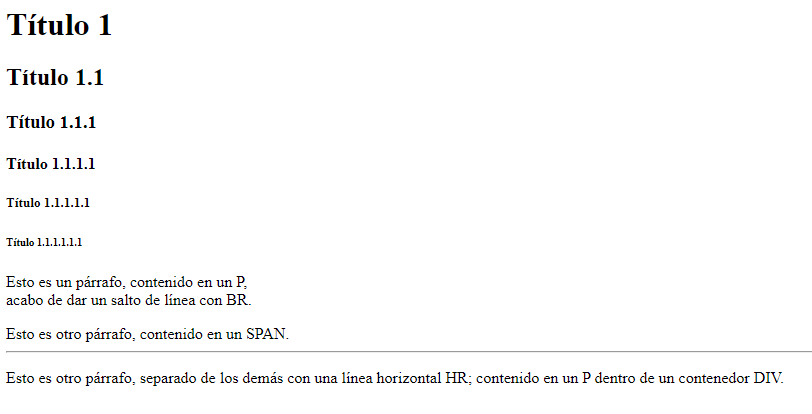
\includegraphics[width=12cm]{ss_html/etiquetas_basicas.png}
\end{figure}


\subsection{Etiquetas de formato}
\begin{itemize}
    \item \textbf{b}: vuelve el texto negrita.
    \item \textbf{big}: vuelve un texto un poco más grande.
    \item \textbf{i}: vuelve el texto cursiva.
    \item \textbf{small}: vuelve el texto un poco más pequeño.
    \item \textbf{strong}: resalta un texto importante con negritas.
    \item \textbf{em}: resalta un texto importante con cursiva.
    \item \textbf{sub}: posiciona un texto en un subíndice.
    \item \textbf{sup}: posiciona un texto en un superíndice.
    \item \textbf{ins}: subraya un texto.
    \item \textbf{del}: tacha un texto.
\end{itemize}

Un ejemplo del aspecto de las etiquetas anteriormente mencionadas es el siguiente código y la \textit{Figura \ref{fig: 2}}:
\begin{lstlisting}
    <b>Este texto es negrita.</b><br/>
    
    <strong>Este texto es negrita e importante para el buscador.</strong><br/>
    
    <i>Este texto es cursiva.</i><br/>
    
    <em>Este texto es cursiva e importante para el buscador.</em><br/>
    
    <ins>Este texto está subrayado.</ins><br/>
    
    <del>Este texto está tachado</del><br/>
    
    <big>Este texto es más grande.</big><br/>
    
    <small>Este texto es más pequeño.</small><br/>
    
    <sup>Este texto tiene un <sup>super índice.</sup><br/>
    
    <sub>Este texto tiene un <sub>sub índice.</sub>
\end{lstlisting}
\begin{figure}[H]
    \centering
    \caption{Vista de las etiquetas de formato}
    \label{fig: 2}
    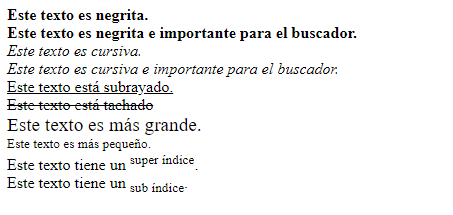
\includegraphics[width=11cm]{ss_html/etiquetas_formato.png}
\end{figure}


\subsection{Atributos de etiquetas}

Son información adicional que modifican a la etiqueta. Estos atributos poseen valores.
\begin{itemize}
    \item \textbf{align}: alinea un texto o etiqueta (img, table, p, texto, h1, etc). Sus posibles valores son:
    \begin{itemize}
        \item \textbf{left}: alinea y justifica a la derecha.
        \item \textbf{center}: alinea y justifica al centro.
        \item \textbf{rigth}: alinea y justifica a la izquierda
        \item \textbf{justify}: justifica el texto.
        \item \textbf{char}: alinea el texto según un carácter.
    \end{itemize}
    \item \textbf{width}: ajusta el ancho de una etiqueta. Las unidades utilizadas para este atributo son el \textit{porcentaje del ancho del sitio o página web o imagen} y los \textit{píxeles}.
    \item \textbf{height}: ajusta el alto de una etiqueta. Las unidades utilizadas para este atributo son el \textit{porcentaje del ancho del sitio o página web o imagen} y los \textit{píxeles}.
    \item \textbf{src}: enlaza links o archivos al sitio o página. Suele ser utilizado con la etiqueta \textit{img} o \textit{a}.
    \item \textbf{alt}: despliega o muestra una imagen o texto alternativo en caso de que el principal no pueda ser mostrado o cargado. Suele ser utilizado con la etiqueta \textit{img} y es \textbf{obligatorio}.
    \item \textbf{border}: agrega un marco o borde a una etiqueta (imagen o tabla). El grosor del borde se establece mediante píxeles. Este atributo puede explotarse más con CSS.
    \item \textbf{bgcolor}: cambia el color de fondo de un elemento.
\end{itemize}

Un ejemplo del aspecto de algunos de los atributos anteriormente mencionados es el siguiente código y la \textit{Figura \ref{fig: 3}}:
\begin{lstlisting}
    <!-- Imagen con distintos atributos. -->
    <img
        align="right" 
        src="https://images.unsplash.com/photo-1593288942460-e321b92a6cde?ixlib=rb-4.0.3&ixid=MnwxMjA3fDB8MHxleHBsb3JlLWZlZWR8Mnx8fGVufDB8fHx8&w=1000&q=80"
        width="700px" 
        height="500px" 
        border="10px" 
        alt="https://images.hola.com/imagenes/mascotas/20180925130054/consejos-para-cuidar-a-un-gatito-recien-nacido-cs/0-601-526/cuidardgatito-t.jpg"/>
\end{lstlisting}
\begin{figure}[H]
    \centering
    \caption{Vista de algunos atributos de etiquetas}
    \label{fig: 3}
    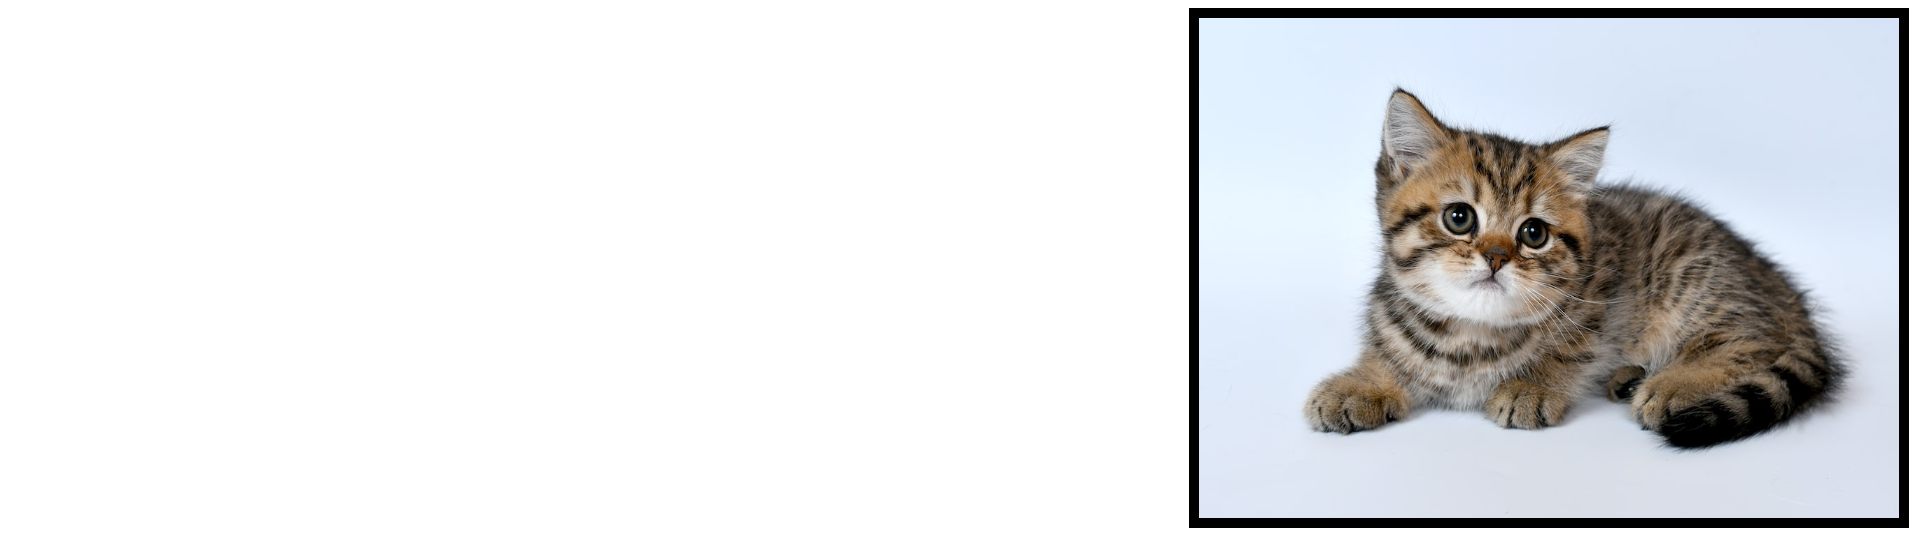
\includegraphics[width=13cm]{ss_html/imgs_atributos.png}
\end{figure}

Vemos que el ejemplo anterior aplica diversos atributos a una etiqueta \textbf{img}, se le asigna una imagen predeterminada y alternativa con los atributos \textit{src} y \textit{alt} respectivamente, un ancho y alto con \textit{width} y \textit{height} y un borde de 10 píxeles con \textit{border}.

Si un atributo choca con otro, es decir, se centra el contenido de una etiqueta \textit{p} y, dentro de este, existe otra etiqueta \textit{p} que alinea el texto a la izquierda, el buscador alineará todas las sub-etiquetas de la etiqueta \textit{p} principal según el atributo de alineación de esta última, y esto aplica para otros tipos de atributos o situaciones.


\subsection{Comentarios}

Un comentario comienza con \textbf{$<$!--} y termina con \textbf{--$>$}:
\begin{center}
    \textit{$<$!-- Esto es un comentario. --$>$}
\end{center}


\subsection{Listas}

Las etiquetas \textbf{ol} y \textbf{ul} generan una lista numerada y no numerada respectivamente. La etiqueta \textbf{li} representa los puntos o elementos de una lista numerada o no numerada.

Si las listas son contenidas dentro de un \textbf{div} o \textbf{p}, se le pueden poner los atributos \textit{align}, \textit{width}, \textit{height} y \textit{border}.

Un ejemplo del aspecto de listas es el siguiente, junto con la \textit{Figura \ref{fig: 4}}:
\begin{lstlisting}
    <h2>Lista numerada</h2>
    <ol>
        <!-- Comienza desde 1. -->
        <li>Opción numerada 1</li>
        <li>Opción numerada 2</li>
        <li>Opción numerada 3</li>
        <li>Opción numerada 4</li>
    </ol>
    <h2>Lista numerada comenzando a partir del 4</h2>
    <ol>
        <!-- Comienza desde 4. -->
        <li value="4">Opción numerada 1</li>
        <li>Opción numerada 2</li>
        <li>Opción numerada 3</li>
        <li>Opción numerada 4</li>
    </ol>
    <h2>Lista no numerada</h2>
    <ul>
        <li>Opción no numerada 1</li>
        <li>Opción no numerada 2</li>
        <li>Opción no numerada 3</li>
        <li>Opción no numerada 4</li>
    </ul>
\end{lstlisting}
\begin{figure}[H]
    \centering
    \caption{Vista las Listas}
    \label{fig: 4}
    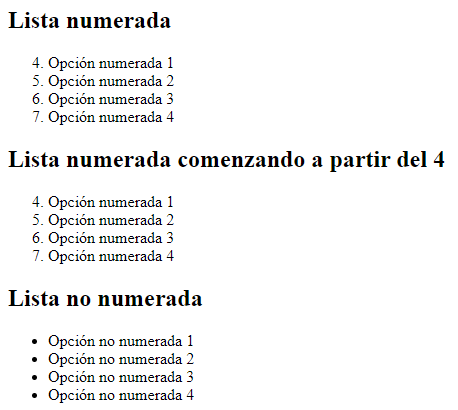
\includegraphics[height=8cm]{ss_html/listas.png}
\end{figure}

\textit{Nota}: este es el aspecto predeterminado de las listas en HTML, antes se le podía dar otro aspecto a ambos tipos de listas con un atributo \textit{type}, sin embargo, este ya no es utilizado, para sustituirlo, se recomienza personalizar o estilizar las listas con CSS.


\subsection{Tablas}

La etiqueta \textbf{table} genera una tabla. Sus sub-etiquetas y atributos son:
\begin{itemize}
    \item \textbf{tr}: etiqueta que representa una fila en la tabla. Dentro de estas, va el contenido, celdas o columnas de cada fila.
    \item \textbf{td}: etiqueta que representa una celda, contenido o columna de una fila de una tabla.
    \item \textbf{th}: etiqueta que representa la cabecera o título de cada columna de una tabla.
    \item \textbf{colspan}: atributo que combina \textit{n} cantidad de columnas o celdas en una tabla.
    \item \textbf{rowspan}: atributo que combina \textit{n} cantidad de filas en una tabla.
    \item Los atributos \textit{align}, \textit{width} y \textit{height} aplican a las etiquetas \textbf{tr} y \textbf{td}.
    \item Los atributos \textit{width}, \textit{height}, \textit{bgcolor} y \textit{border} aplican a la esta etiqueta y a las sub-etiquetas.
\end{itemize}

Un ejemplo del aspecto de las tablas es el siguiente, junto con la \textit{Figura \ref{fig: 5}}:
\begin{lstlisting}
    <h2>Tabla regular</h2>
    <!-- Borde de 2 píxeles, ancho y alto de 200 píxeles. -->
    <table border="2px" width="200px" height="200px">
        <!-- Elementos alineados al centro. -->
        <tr align="center">
            <td>1</td>
            <td>2</td>
            <td>3</td>
        </tr>
        <tr align="center">
            <td>4</td>
            <td>5</td>
            <td>6</td>
        </tr>
        <tr align="center">
            <td>7</td>
            <td>8</td>
            <td>9</td>
        </tr>
    </table>
    <h2>Tabla con columnas combinadas</h2>
    <table border="2px" width="200px" height="200px">
        <tr align="center">
            <!-- Crea dos celdas que combinan dos columnas. -->
            <td colspan="2">1</td>
            <td colspan="2">2</td>
        </tr>
        <tr align="center">
            <td>3</td>
            <td>4</td>
            <td>5</td>
            <td>6</td>
        </tr>
        <tr align="center">
            <td>7</td>
            <td>8</td>
            <td>9</td>
            <td>10</td>
            </tr>
    </table>
    <h2>Tabla con filas combinadas</h2>
    <table border="2px" width="200px" height="200px">
        <tr align="center">
            <!-- Crea una fila que combina tres celdas. -->
            <td rowspan="3">1</td>
            <td>2</td>
            <td>3</td>
            <td>4</td>
        </tr>
        <tr align="center">
            <td>7</td>
            <td>5</td>
            <td>6</td>
        </tr>
        <tr align="center">
            <td>8</td>
            <td>9</td>
            <td>10</td>
        </tr>
    </table>
\end{lstlisting}
\begin{figure}[H]
    \centering
    \caption{Vista las Tablas}
    \label{fig: 5}
    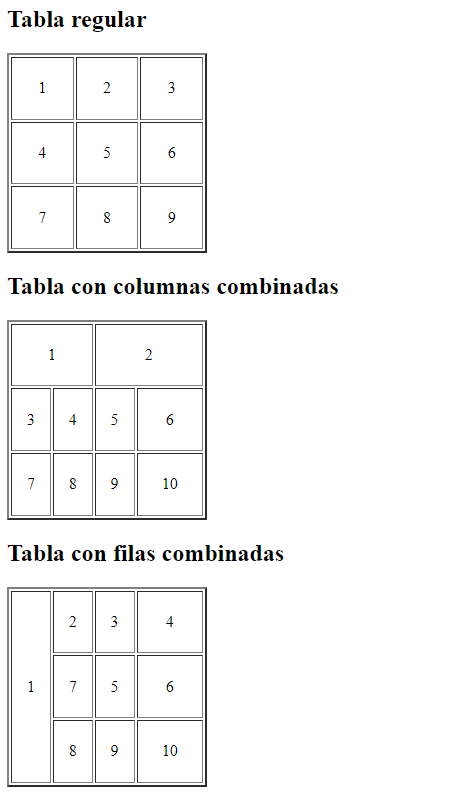
\includegraphics[height=12cm]{ss_html/tablas.png}
\end{figure}

Vemos que el ejemplo anterior posee tres tablas, con un borde de 2 píxeles, con todo su contenido alineado al centro y con un tamaño de ancho y alto de 200 píxeles, la primer tabla es una tabla regular de 3x3, la segunda tabla combina dos y dos columnas y la tercer tabla combina tres filas.


\subsection{Imágenes}

Enlaza una imagen al sitio o página web con la etiqueta \textbf{img}. \textbf{Esta etiqueta no requiere una etiqueta de cierre}. Las imágenes son pesadas, es recomendado utilizar imágenes del tamaño que se deseen o requieran mostrar, ni tan grandes ni tan pequeñas, y en el formato adecuado (.jpg, .png u otros). Sus atributos son:
\begin{itemize}
    \item \textbf{src}: la ruta o dirección web de la imagen.
    \item \textbf{alt}: el texto o imagen alternativo en caso de que la imagen principal no cargue.
    \item Los atributos \textit{align}, \textit{height}, \textit{width} y \textit{border} aplican a esta etiqueta.
\end{itemize}

El uso de imágenes ya se vio en la Figura \ref{fig: 3}.


\subsection{Enlaces}

Enlaza a un documento, imagen, archivo, sitio o página o dirección web con la etiqueta \textbf{a}. Sus atributos son:
\begin{itemize}
    \item \textbf{href}: es el enlace a donde se redireccionará.
    \item \textbf{target}: establece como dónde y cómo se abrirá el enlace o documento. Sus posibles valores son:
    \begin{itemize}
        \item \textbf{\_blank}: carga en una nueva pestaña.
        \item \textbf{\_self}: carga en el actual \textit{frame}.
        \item \textbf{\_parent}: carga en el \textit{frame} padre o del \textit{frame} actual.
        \item \textbf{\_top}: carga en la pestaña actual.
        \item \textbf{framename}: carga en un \textit{frame} determinado.
    \end{itemize}
    \item El atributo \textit{align} aplica a esta etiqueta.
\end{itemize}

Un ejemplo del aspecto de los enlaces es el siguiente, junto con la \textit{Figura \ref{fig: 6}}, donde se muestra el aspecto del enlace antes de dar clic en él, la \textit{Figura \ref{fig: 7}} muestra que se ha abierto otra pestaña después de haber dado clic en el enlace:
\begin{lstlisting}
    <a href="https://github.com/migueluisV" target="_blank">Github</a>
\end{lstlisting}
\begin{figure}[H]
    \centering
    \caption{Vista de Enlaces previo al clic}
    \label{fig: 6}
    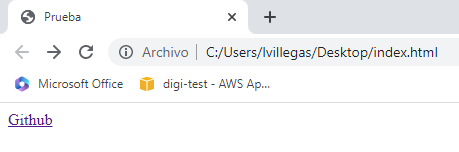
\includegraphics[width=11cm]{ss_html/enlaces_1.png}
\end{figure}
\begin{figure}[H]
    \centering
    \caption{Vista de Enlaces después del clic}
    \label{fig: 7}
    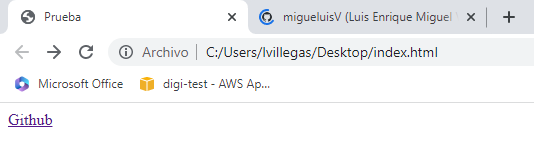
\includegraphics[width=11cm]{ss_html/enlaces_2.png}
\end{figure}

Al enlace se le configuró el atributo \textit{target} con el valor \textbf{\_blank} para que se abriera el enlace en una nueva pestaña, puede probar con los otros valores de este atributo para ver el comportamiento.


\subsection{Formularios}

La etiqueta \textbf{form} crea un formulario para recolectar información del usuario, esta información es enviada a un servidor u otro sitio o página, siendo procesada por un lenguaje de programación (PHP o JavaScript por ejemplo). Sus sub-etiquetas y atributos son:
\begin{itemize}
    \item \textbf{input}: etiqueta que crea un control para que el usuario interactúe con el. Sus atributos son:
    \begin{itemize}
        \item \textbf{type}: es el tipo de control a generar. Sus posibles valores son:
        \begin{itemize}
            \item \textbf{text}: caja de texto.
            \item \textbf{password}: caja de texto con caracteres especiales para proteger texto.
            \item \textbf{radio}: RadioButton.
            \item \textbf{checkbox}: caja de marcado.
            \item \textbf{submit}: botón que envía la información del formulario.
        \end{itemize}
        \item \textbf{placeholder}: texto por defecto que se muestra en una caja de texto.
        \item \textbf{name}: nombre único del control.
        \item \textbf{value}: el valor que almacena el control, se suele aplicar a \textit{submit}, \textit{radio} y \textit{checkbox}.
    \end{itemize}
    \item \textbf{textarea}: caja de texto multilínea. Tiene un inicio y final.
    \begin{itemize}
        \item \textbf{rows}: indica las filas por defecto de la textarea.
        \item \textbf{cols}: indica las columnas por defecto de la textarea.
        \item Los atributos \textit{name} y \textit{placeholder} aplican a esta etiqueta.
    \end{itemize}
    \item \textbf{action}: atributo de \textbf{form} que carga una dirección web una vez se llenó y envió el formulario. Si se le pone el valor \textbf{\#} a este atributo, el formulario cargará la página donde está contenido (se refrescará la página sin cambio alguno).
    \item \textbf{method}: atributo de \textbf{form} especifica el método HTTP cuando el formulario es enviado. Sus posibles valores son:
    \begin{itemize}
        \item \textbf{GET}: la información recolectada puede verse en la dirección web del sitio a donde fue mandada.
        \item \textbf{POST}: la información no es visible, y ofrece mejor seguridad si es que la información es sensible o se está actualizando.
    \end{itemize}
    \item Dependiendo de cómo se presente el formulario (con \textbf{div}, \textbf{span}, \textbf{p} u otros), se le pueden aplicar los atributos más populares anteriormente vistos.
\end{itemize}

Un ejemplo del aspecto de los enlaces es el siguiente, junto con la \textit{Figura \ref{fig: 8}}:
\begin{lstlisting}
    <form action="#" method="POST">
        p>Caja de texto: </p><input type="text" name="txt1" placeholder="Ingresa un texto..." />
        
        <p>Caja de texto multi línea: </p><textarea name="txta1" rows="10" cols="50" placeholder="Ingresa un texto..."></textarea>
        
        <p>Contraseña: </p><input type="password" name="psw1" />
        
        <p>RadioButtons: </p>
        <input type="radio" name="rb1" value="1" />Valor 1
        <br/>
        <input type="radio" name="rb1" value="2" />Valor 2
        
        <p>Checkbox: </p>
        <input type="checkbox" name="chb1" value="3" />Opción 1
        <br/>
        
        <input type="checkbox" name="chb2" value="4" />Opción 2
        
        <p>Botones: </p><input type="submit" name="btn1" value="Enviar" />
    </form>
\end{lstlisting}
\begin{figure}[H]
    \centering
    \caption{Vista de los Formularios}
    \label{fig: 8}
    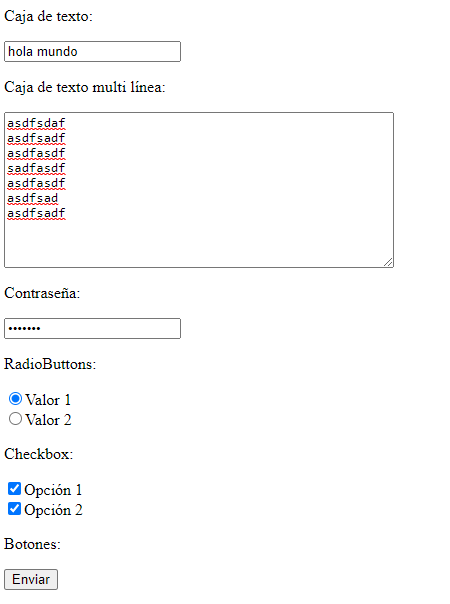
\includegraphics[height=12cm]{ss_html/formularios.png}
\end{figure}

Se creó un formulario con una caja de texto, una caja de texto multilínea, una caja para contraseñas, dos opciones de RadioButtons, dos opciones de CheckBoxs y un botón que envía la información recaba al mismo sitio. El formulario tiene el atributo \textit{action} y \textit{method} con los valores \textbf{\#} y \textbf{POST} respectivamente, envía la información protegida al mismo sitio donde está contenido el formulario. Algunas cajas de texto tienen el atributo \textit{placeholder}, para que se muestre un texto predeterminado que se elimina una vez el usuario ingresa algún texto. El control textarea posee los atributos \textit{rows} y \textit{cols} para mostrar una cantidad determinada de filas y columnas respectivamente, esto para resaltar que es un control multilínea.

Fíjese que el nombre de los dos RadioButtons utilizados es el mismo, esto es así ya que este control solo permite seleccionar una opción, si tuviéramos dos o más RadioButtons con distinto nombre, se podrían seleccionar todos sin problema; esto no ocurre con los CheckBoxs.

Todos los controles utilizados en el ejemplo anterior poseen su nombre único con el atributo \textit{name}; \textbf{existen más controles}.


\subsection{Frames}

Los \textbf{frames} son contenedores donde podemos almacenar distintas páginas o contenido dentro de una sola ventana o página. El \textbf{frameset} es la etiqueta Block-Level de los \textbf{frames}, esta define cuantos frames habrá en el frameset (columnas y filas), su espacio definido, borde, etc.

Esta etiqueta o estructura ya no está soportada en HTML5. \textbf{frameset} sustituye la etiqueta \textbf{body} en un documento HTML. Algunos de sus atributos son:
\begin{itemize}
    \item \textbf{cols}: atributo que establece en cuántas columnas se seccionará la página web. El tamaño de estas columnas se determina por porcentajes o píxeles.
    \item \textbf{rows}: atributo que establece en cuántas filas se seccionará la página web. El tamaño de estas filas se determina por porcentajes o píxeles.
    \item \textbf{src}: atributo que determina el archivo o sitio web que se cargará en el frame.
    \item \textbf{noresize}: atributo que indica que un frame no puede cambiar su tamaño.
    \item \textbf{noframe}: etiqueta que indica al buscador que la página o sitio no soporta frames.
\end{itemize}

Veamos un ejemplo tomado de internet modificado por nosotros enseguida, en la \textit{Figura \ref{fig: 9}}:
\begin{lstlisting}
    <html>
        <head>
            <title>Un documento simple con marcos</title>
        </head>
        <frameset rows="20%,80%">
            <frameset cols="20%, 80%">
                <frame src="https://images.hola.com/imagenes/mascotas/20180925130054/consejos-para-cuidar-a-un-gatito-recien-nacido-cs/0-601-526/cuidardgatito-t.jpg">
                <frame src="https://images.unsplash.com/photo-1593288942460-e321b92a6cde?ixlib=rb-4.0.3&ixid=MnwxMjA3fDB8MHxleHBsb3JlLWZlZWR8Mnx8fGVufDB8fHx8&w=1000&q=80">
            </frameset>
            <frame src="https://images.unsplash.com/photo-1591871937631-2f64059d234f?ixlib=rb-4.0.3&ixid=MnwxMjA3fDB8MHxleHBsb3JlLWZlZWR8MXx8fGVufDB8fHx8&w=1000&q=80">
        </frameset>
    </html>
\end{lstlisting}
\begin{figure}[H]
    \centering
    \caption{Vista de los Framesets}
    \label{fig: 9}
    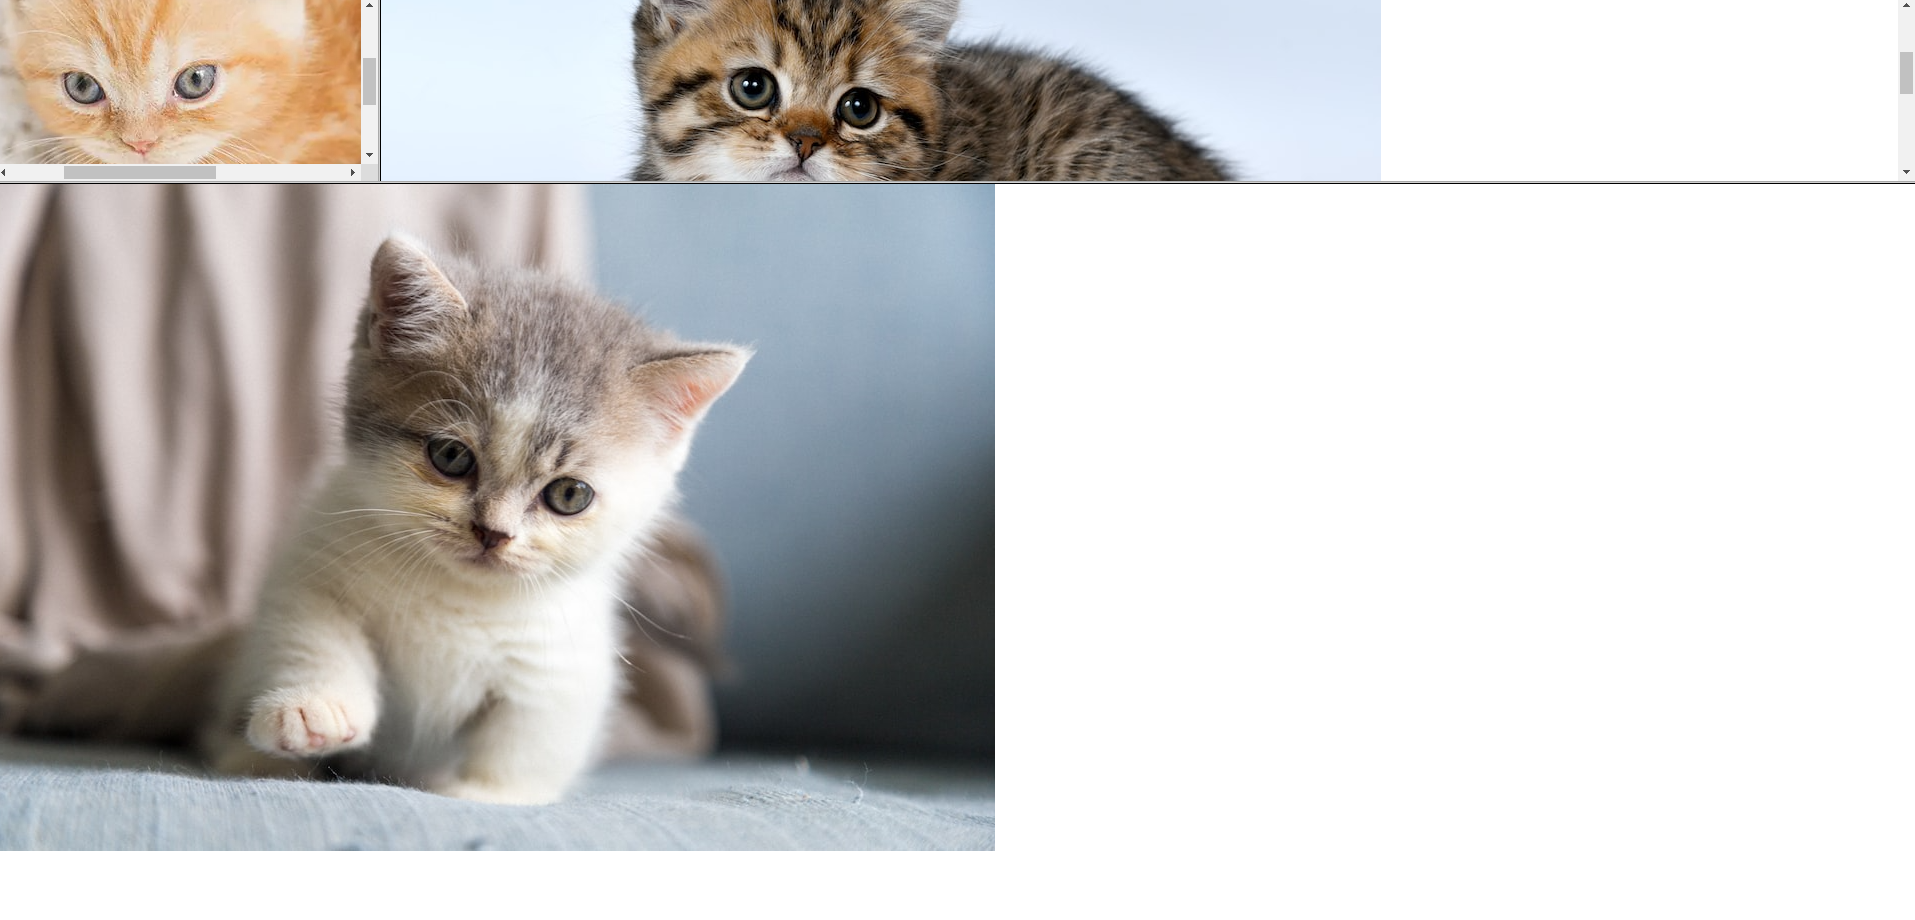
\includegraphics[width=13cm]{ss_html/frames_1.png}
\end{figure}

El ejemplo presenta un \textbf{frameset} principal que contiene dos columnas, una del tamaño del 20\% de la pantalla y la otra del 80\%: el primer \textbf{frame} contiene otro \textit{frameset} con dos filas, igual con tamaños de 20 y 80 porciento, así combinamos el uso de framesets. El principal pose un borde de 3 píxeles, que afecta al resto de frames o framesets internos, vemos que aquellos que requieren de desplazamiento se les inserta automáticamente barras deslizadoras para recorrer el frame, si ponemos el puntero en los bordes, estos pueden ser redimensionados, como se ve en la \textit{Figura \ref{fig: 10}}:
\begin{figure}[H]
    \begin{center}
        \caption{Vista de los Framesets redimensionados}
        \label{fig: 10}
        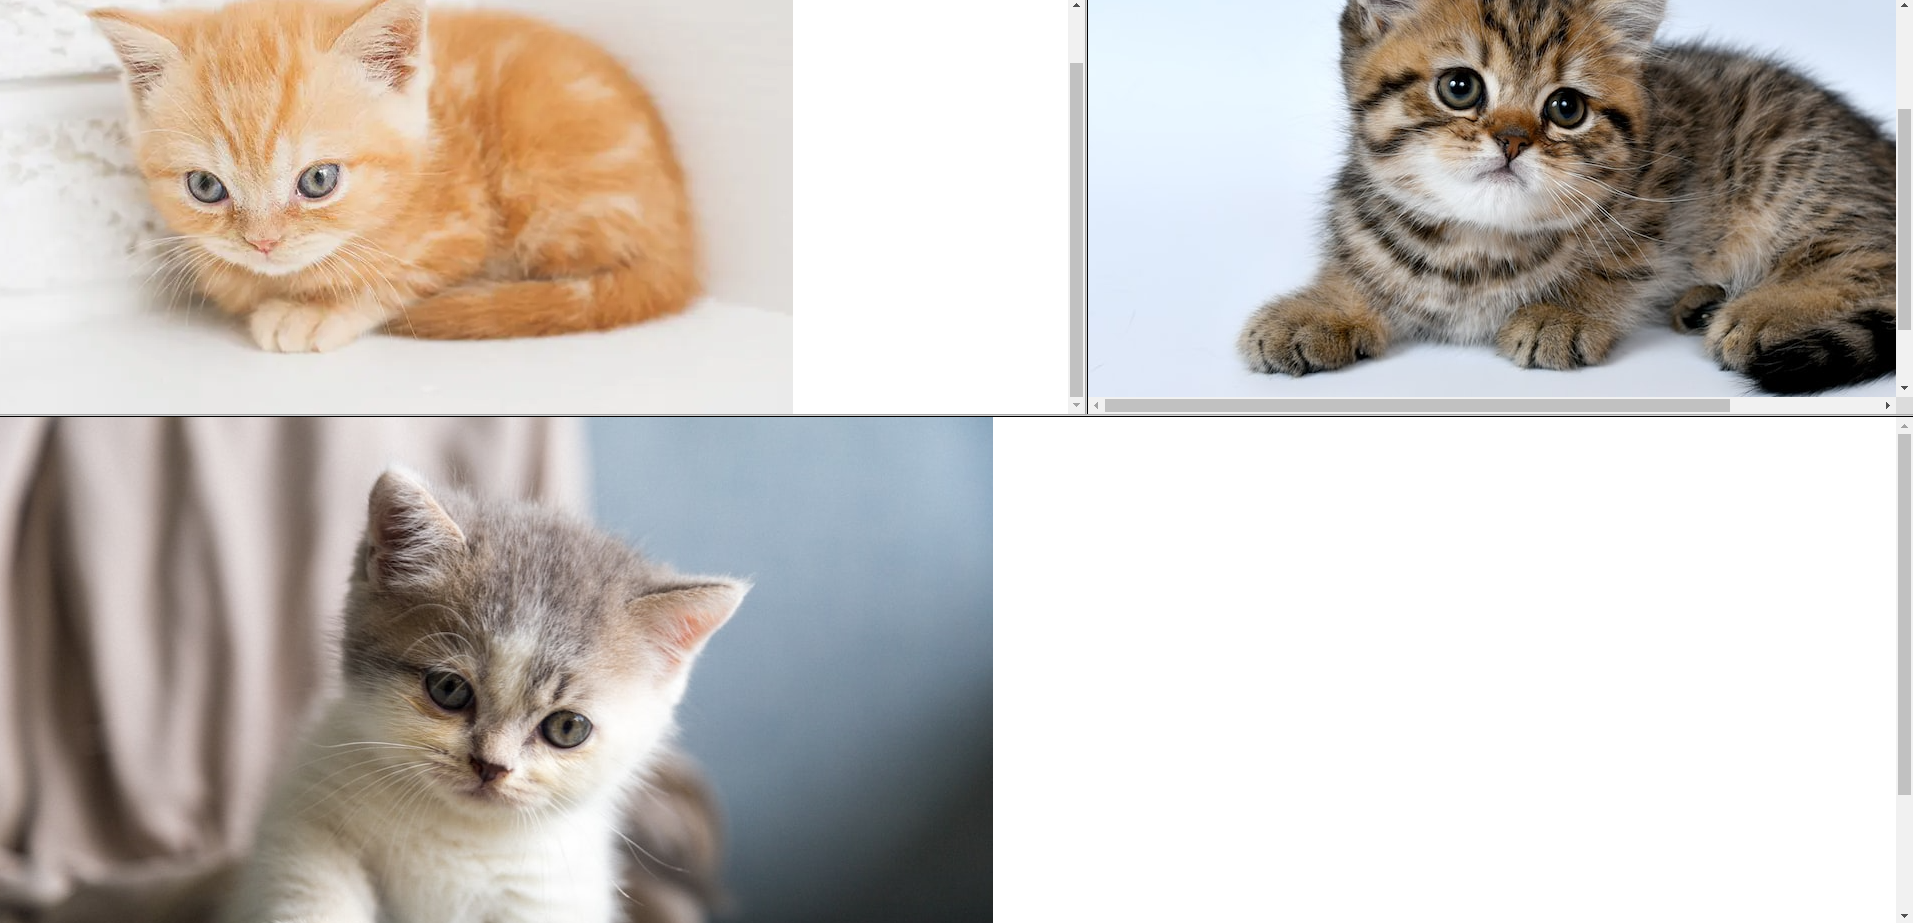
\includegraphics[width=13cm]{ss_html/frames_2.png}
    \end{center}
\end{figure}

En caso de que no se requiera la posibilidad de redimensionamiento de frames, aplicar el atributo \textit{noresize}. \textbf{frameset ya no es soportado por HTML5}.


\subsection{Colores}

Los colores son representados como valores hexadecimales:
\begin{center}
    0, 1, 2, 3, 4, 5, 6, 7, 8, 9, A, B, C, D, E, F
\end{center}

Los colores en HTML son desplegados según el modelo RGB (Red, Green, Blue), para escribir un color es necesario escribir el símbolo de gato (\#), seguido de su código de combinación de tres o seis, como vemos el la \textit{Figura \ref{fig: 11}}:
\begin{figure}[H]
    \centering
    \caption{Ejemplo de colores HTML}
    \label{fig: 11}
    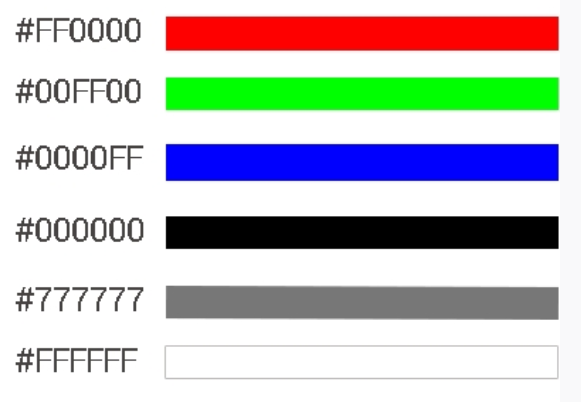
\includegraphics[width=7cm]{ss_html/ejemplo_colores.png}
\end{figure}
